

%%%%%%%%%%%%%%%%%%%%%%%%%%%%%%%%%%%%%%%%%%%%%%%%%%%%%%%%%%%%%%%%%%%%%%%%%%%%%%%%%%%%%%%%%%%%%%%%%%%%%%%%%%%%%
\subsection{Additional Results for Preliminary Study - Section~\ref{sec:pre2}}\label{app:pre2}

In this subsection, we provide more experimental results to validate the statement 
in Section~\ref{sec:pre2}, where we state that fitting atypical samples in adversarial training can hurt the performance (clean \& adversarial accuracy) of typical samples.
We provide full empirical results to show that: \textbf{(i)} In traditional ERM, fitting atypical samples will not hurt the models' performance (clean accuracy) of typical samples. \textbf{(ii)} In adversarial training, fitting atypical samples can degrade the clean \& adversarial accuracy of typical samples. \textbf{(iii)} In adversarial training, fitting atypical samples can degrade the quality of learned representations, especially the models' discrimination between classes.
The experimental setting follows Section~\ref{sec:pre2}, where we train the models for several trails on resampled (CIFAR100, CIFAR10, Tiny~ImageNet) datasets: each dataset is constructed with the whole training typical set $\mathcal{D}_\text{typ}$, and a part of the training atypical set $\mathcal{D}_\text{atyp}$ (randomly sample 0\%, 20\% and 100\% in $\mathcal{D}_\text{atyp}$). We evaluate the models' performance on test ``typical'' set $\mathcal{D}'_\text{typ}$ which is defined in Section~\ref{sec:pre2}.

\newpage
\textbf{(i) Additional Results for Preliminary Study - Section~\ref{sec:pre2} In Traditional ERM}

Fig.~\ref{fig:app2_11}, Fig.~\ref{fig:app2_12} and Fig.~\ref{fig:app2_13} report the performance of traditional ERM, trained on different resampled datasets with different amount of atypical samples existed. The figures report the clean accuracy on test typical set of CIFAR100, CIFAR10 and Tiny~ImageNet. We also leave the robustness performance out here as the models are not robust to adversarial attacks. From the results, we can conclude that in traditional ERM, fitting atypical samples will not degrade the models' performance on typical samples. For example, in CIFAR100 dataset, with 100\% atypical samples included (Atypical-100\%)., the accuracy on the test typical set is even slightly higher than the model trained without atypical samples (Atypical-0\%). This conclusion is consistent for all three datasets and model architectures.


\begin{figure}[h]
\centering
\hspace*{-1cm}
\subfloat[ResNet18.]{
\begin{minipage}[c]{0.3\textwidth}
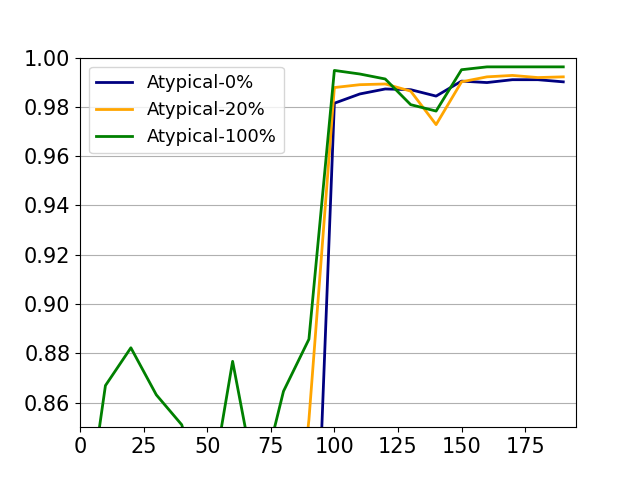
\includegraphics[width = 1.0\textwidth]{figures/pre2_clean_cifar100_ResNet18.png}
\end{minipage}
}
\hspace*{0.4cm}
\subfloat[WRN28.]{
\begin{minipage}[c]{0.3\textwidth}
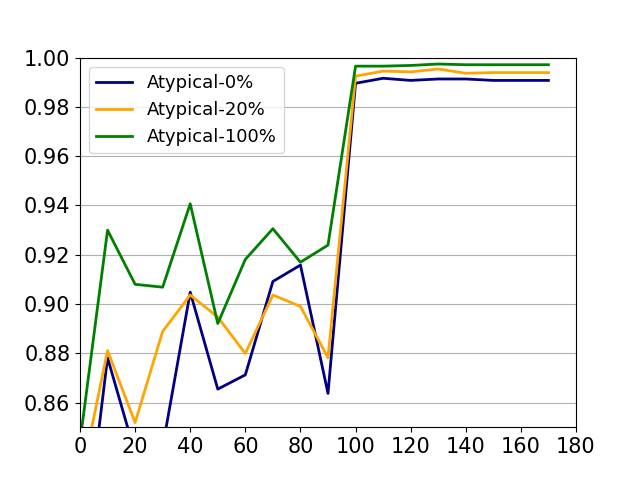
\includegraphics[width = 1.0\textwidth]{figures/pre2_clean_cifar100_WRN28.png}%
\end{minipage}
}
\caption{Clean Accuracy on \textbf{Typical} Set of CIFAR100}
\label{fig:app2_11}
\vspace{-0.5cm}
\end{figure}
%%%%%%%%%%%%%%%%%%%%%%%%%%%%%%%%%%%
\begin{figure}[h]
\centering
\hspace*{-1cm}
\subfloat[ResNet18.]{
\begin{minipage}[c]{0.3\textwidth}
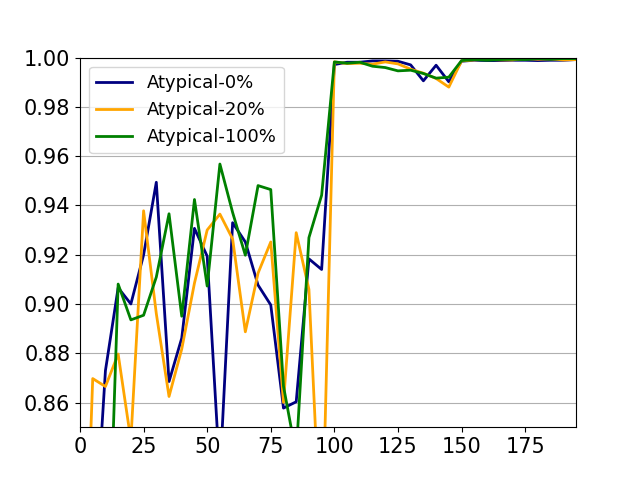
\includegraphics[width = 1.0\textwidth]{figures/pre2_clean_cifar10_ResNet18.png}
\end{minipage}
}
\hspace*{0.4cm}
\subfloat[WRN28.]{
\begin{minipage}[c]{0.3\textwidth}
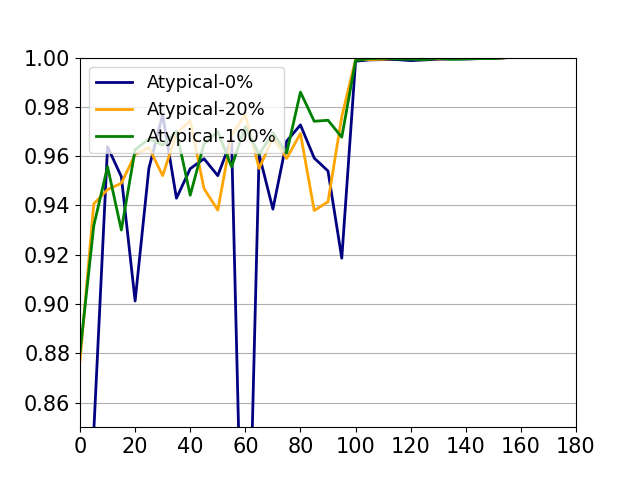
\includegraphics[width = 1.0\textwidth]{figures/pre2_clean_cifar10_WRN28.png}%
\end{minipage}
}
\caption{Clean Accuracy on \textbf{Typical} Set of CIFAR10}
\label{fig:app2_12}
\vspace{-0.5cm}
\end{figure}
%%%%%%%%%%%%%%%%%%%%%%%%%%%%%%%%%%%
\begin{figure}[h!]
\centering
\hspace*{-1cm}
\subfloat[ResNet32.]{
\begin{minipage}[c]{0.3\textwidth}
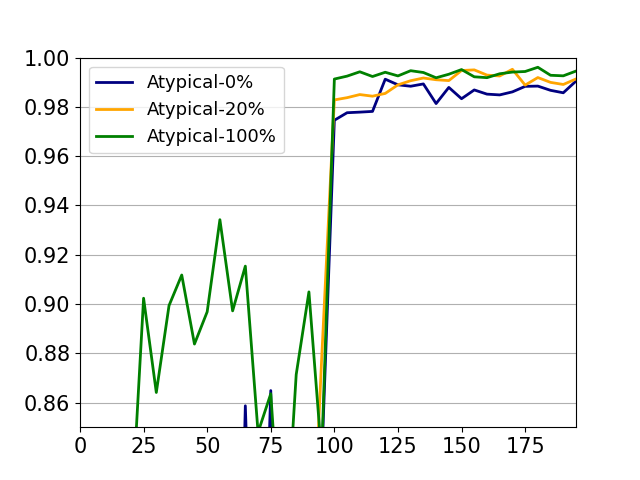
\includegraphics[width = 1.0\textwidth]{figures/pre2_clean_imagenet_ResNet18.png}
\end{minipage}
}
\hspace*{0.4cm}
\subfloat[WRN28.]{
\begin{minipage}[c]{0.3\textwidth}
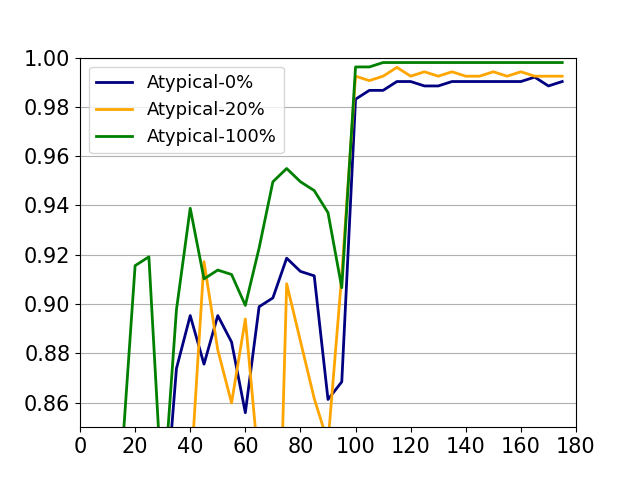
\includegraphics[width = 1.0\textwidth]{figures/pre2_clean_imagenet_WRN28.png}%
\end{minipage}
}
\caption{Clean Accuracy on \textbf{Typical} Set of Tiny~ImageNet}
\label{fig:app2_13}
\end{figure}





%%%%%%%%%%%%%%%%%%%%%%%%%%%%%%%%%%%%%%%%%%%%%%%%%%%%%%%%%%%%%%%%%%%%%%%%%%%%%%%%%%%%%%%%%%%%%%%%%%%%%%%%%%%%%%%%%%%%%%%%%%%%%%%%%%%%%%%%%%%%%%%%%%%%%%%%%%%%%%%%%%%%%%%%%%%%%%%%%%%%%%%%%%
\textbf{(ii) Additional Results for Preliminary Study - Section~\ref{sec:pre2} In Adversarial Training}

Fig.~\ref{fig:pre2_21}, Fig.~\ref{fig:pre2_22} and Fig.~\ref{fig:pre2_23} report the performance of adversarial training, on different resampled datasets with different amount of atypical samples existed. The figures report both clean and adversarial accuracy on test atypical sets of CIFAR100, CIFAR10 and Tiny~ImageNet. Based on the experimental results, we find that including more atypical samples can cause the model have worse performance on typical samples in all three datasets. In datasets with a large portion of atypical samples, such as CIFAR100, the negative effects of atypical samples are more obvious. In CIFAR100, training on datasets with 100\% atypical samples (Atypical 100\%) can cause the clean \& adversarial accuracy drop by $\sim7\%$ and $8\%$, respectively.

\begin{figure}[h]
\centering
\hspace*{-1cm}
\subfloat[Clean (left) \& Adv Acc. (right) under ResNet18.]{
\begin{minipage}[h]{0.55\textwidth}
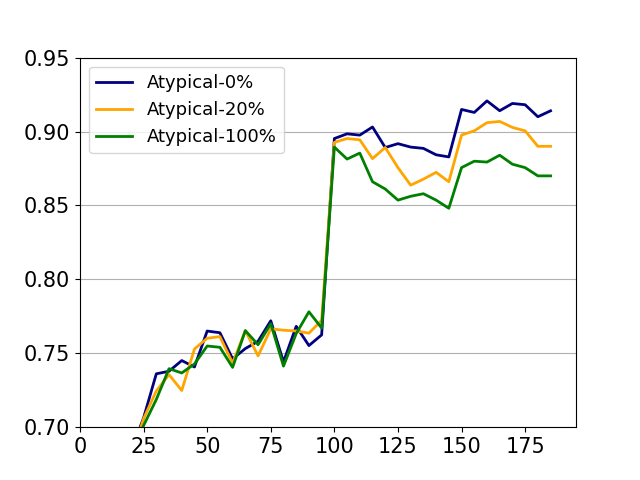
\includegraphics[width = 0.5\textwidth]{figures/poison_clean_ResNet18.png}%
\hfill
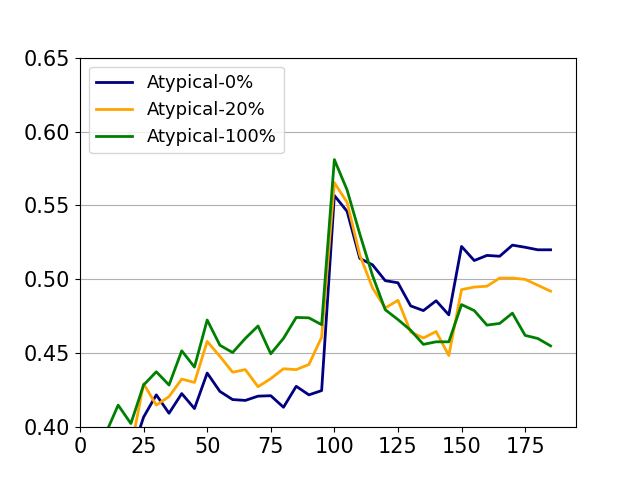
\includegraphics[width = 0.5\textwidth]{figures/poison_adv_ResNet18.png}
\end{minipage}
}
\hspace*{-0.4cm}
\subfloat[Clean (left) \& Adv Acc. (right) under WRN28.]{
\begin{minipage}[c]{0.55\textwidth}
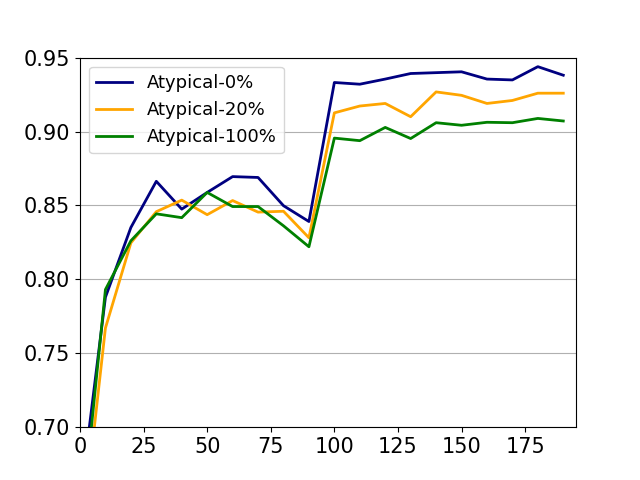
\includegraphics[width = 0.5\textwidth]{figures/poison_clean_WRN.png}%
\hfill
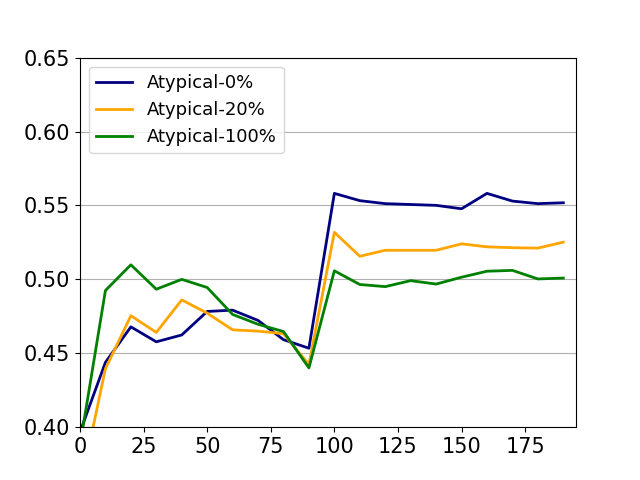
\includegraphics[width = 0.5\textwidth]{figures/poison_adv_WRN.png}
\end{minipage}
}
\caption{Clean Accuracy and Adversarial Accuracy on \textbf{Typical} Set of CIFAR100}
\label{fig:pre2_21}
\vspace{-0.3cm}
\end{figure}
%%%%%%%%%%%%%%%%%%%%%%%%%%%%%%%%%%%%%%%%%%
\begin{figure}[h]
\centering
\hspace*{-1cm}
\subfloat[Clean (left) \& Adv Acc. (right) under ResNet18.]{
\begin{minipage}[h]{0.55\textwidth}
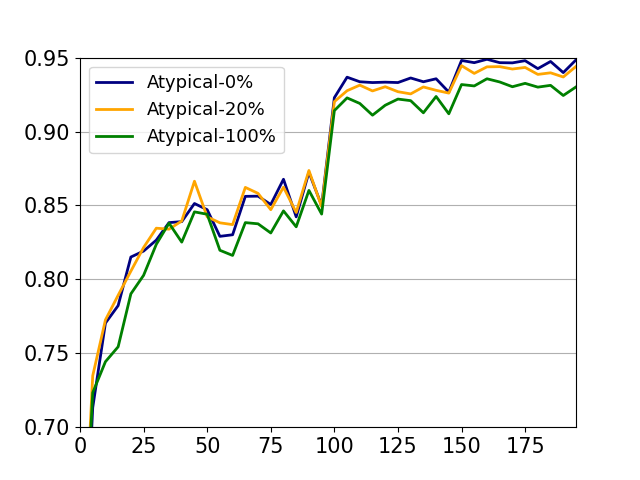
\includegraphics[width = 0.5\textwidth]{figures/pre3_cifar10_adv1_resnet18.png}%
\hfill
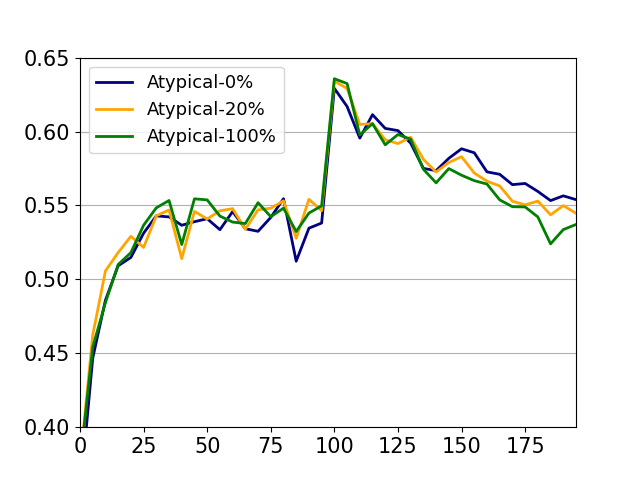
\includegraphics[width = 0.5\textwidth]{figures/pre3_cifar10_adv2_resnet18.png}
\end{minipage}
}
\hspace*{-0.4cm}
\subfloat[Clean (left) \& Adv Acc. (right) under WRN28.]{
\begin{minipage}[c]{0.55\textwidth}
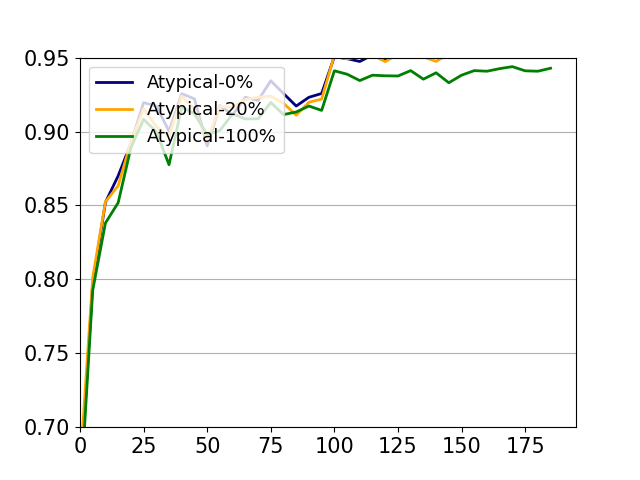
\includegraphics[width = 0.5\textwidth]{figures/pre3_cifar10_adv1_wrn28.png}%
\hfill
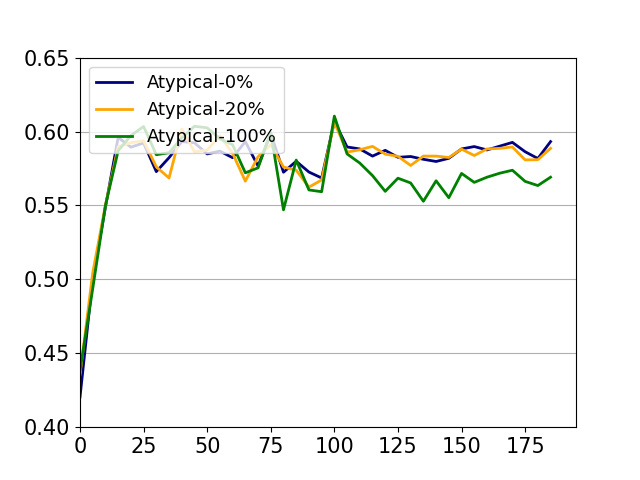
\includegraphics[width = 0.5\textwidth]{figures/pre3_cifar10_adv2_wrn28.png}
\end{minipage}
}
\caption{Clean Accuracy and Adversarial Accuracy on \textbf{Typical} Set of CIFAR10}
\label{fig:pre2_22}
\vspace{-0.3cm}
\end{figure}
%%%%%%%%%%%%%%%%%%%%%%%%%%%%%%%%%%%%%%%%%%
\begin{figure}[h!]
\centering
\hspace*{-1cm}
\subfloat[Clean (left) \& Adv Acc. (right) under ResNet32.]{
\begin{minipage}[h]{0.55\textwidth}
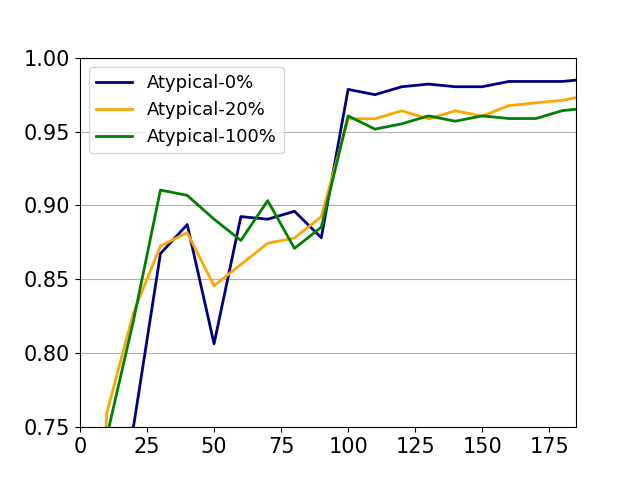
\includegraphics[width = 0.5\textwidth]{figures/pre3_imagenet_adv1_resnet18.png}%
\hfill
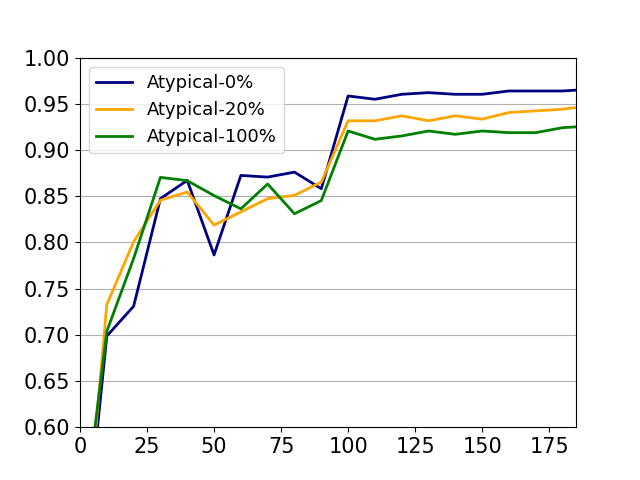
\includegraphics[width = 0.5\textwidth]{figures/pre3_imagenet_adv2_resnet18.png}
\end{minipage}
}
\hspace*{-0.4cm}
\subfloat[Clean (left) \& Adv Acc. (right) under WRN28.]{
\begin{minipage}[c]{0.55\textwidth}
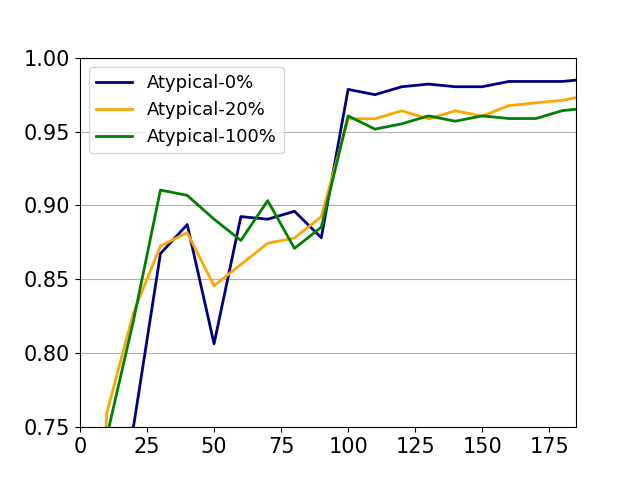
\includegraphics[width = 0.5\textwidth]{figures/pre3_imagenet_adv1_resnet18.png}%
\hfill
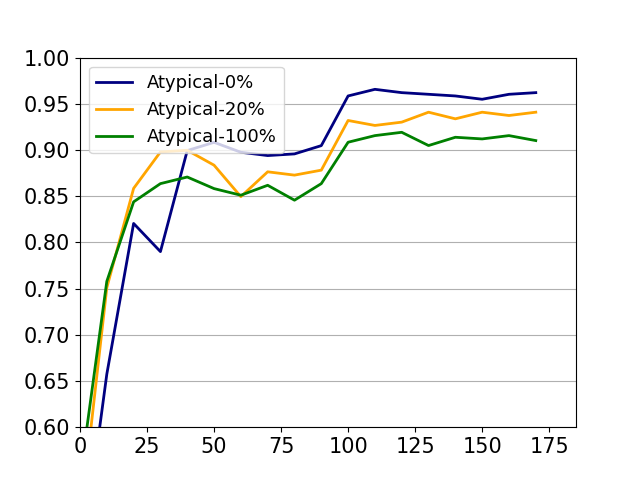
\includegraphics[width = 0.5\textwidth]{figures/pre3_imagenet_adv2_wrn28.png}
\end{minipage}
}
\caption{Clean Accuracy and Adversarial Accuracy on \textbf{Typical} Set of CIFAR100}
\label{fig:pre2_23}
\end{figure}


\vspace{2cm}
\textbf{(iii) Additional Results for Preliminary Study - Section~\ref{sec:pre2} Classwise Representation Distance}

Here, we provide additional evidence to show that in adversarial training, fitting atypical samples can degrade the quality of DNN's learned representations (as proposed in Section~\ref{sec:pre2}). In Fig.~\ref{fig:dist1}, Fig.~\ref{fig:dist2} and Fig.~\ref{fig:dist3}, we measure the Cosine Distance (defined in Section~\ref{sec:pre2}) of the representations for (typical) samples from different classes. In these figures, we provide detailed results of both traditional ERM and adversarial training under ResNet18 and WRN28. From the results, we can see that in adversarial training, more atypical samples can cause the smaller classwise Cosine Distance of the models (on their last epochs). Moreover, during the training process of adversarial training, the classwise Cosine Distance first increases and then starts to decrease, especially when there are more atypical samples are fitted. For example, in CIFAR100 under ResNet18, the Cosine Distance starts to decrease at around Epoch 100, which is when many more atypical samples are fitted. These results suggest that, in adversarial training, fitting atypical samples can be an important reason to cause the models to produce poor representations. As a comparison, in Traditional ERM, the classwise Cosine Distance keeps increasing from the first epoch to the last one. Although given the same epoch, the models trained with more atypical samples also have smaller Cosine Distance, they would not harm the model's final performance. It is because the models trained with more atypical samples can also have relatively large classwise Cosine Distance in their last epochs.


%%%%%%%%%%%%%%%%%%%%%%%%%%%%
\begin{figure}[h]
\centering
\hspace*{-1cm}
\subfloat[Traditional ERM under ResNet18 (left), WRN28 (right).]{
\begin{minipage}[h]{0.55\textwidth}
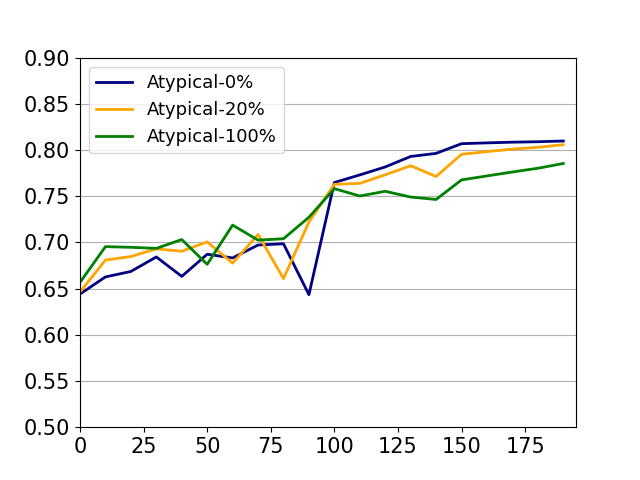
\includegraphics[width = 0.5\textwidth]{figures/dist_cifar100_ResNet18.png}%
\hfill
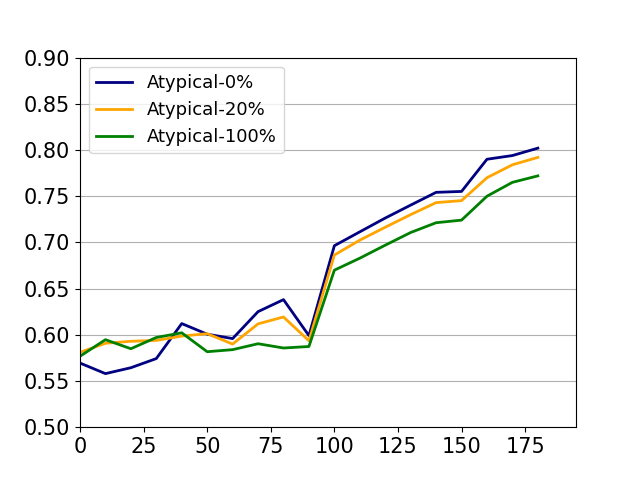
\includegraphics[width = 0.5\textwidth]{figures/dist_cifar100_wrn28.png}
\end{minipage}
}
\hspace*{-0.4cm}
\subfloat[Adv. Training under ResNet18 (left), WRN28 (right).]{
\begin{minipage}[c]{0.55\textwidth}
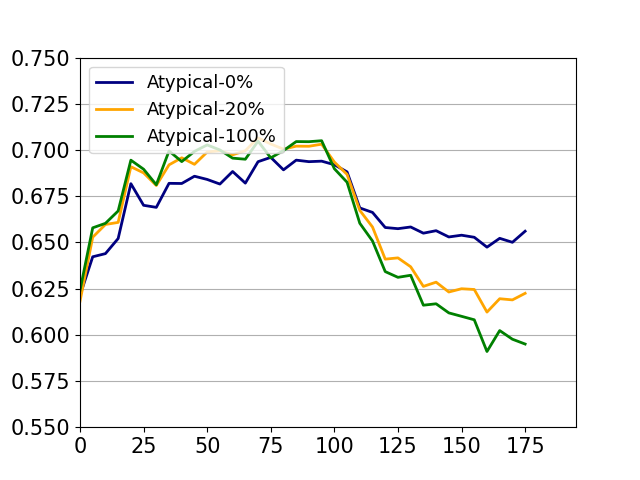
\includegraphics[width = 0.5\textwidth]{figures/dist_adv_cifar100_ResNet18.png}%
\hfill
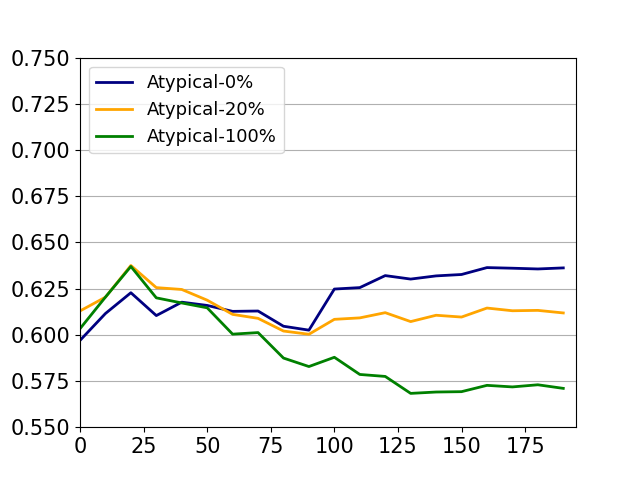
\includegraphics[width = 0.5\textwidth]{figures/dist_adv_cifar100_WRN28.png}
\end{minipage}
}
\caption{Classwise Cosine Distance of Output Representation of \textbf{Typical} Set of CIFAR100}
\label{fig:dist1}
\end{figure}

%%%%%%%%%%%%%%%%%%%%%%%%%%%%
\begin{figure}[h]
\centering
\hspace*{-1cm}
\subfloat[Traditional ERM under ResNet18 (left), WRN28 (right).]{
\begin{minipage}[h]{0.55\textwidth}
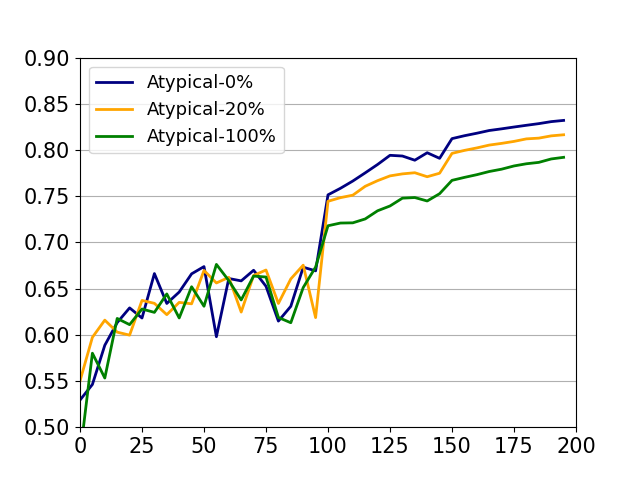
\includegraphics[width = 0.5\textwidth]{figures/dist_cifar10_ResNet18.png}%
\hfill
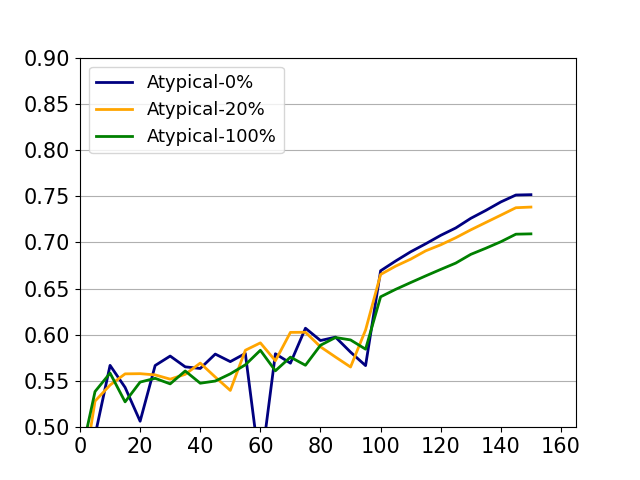
\includegraphics[width = 0.5\textwidth]{figures/dist_cifar10_WRN28.png}
\end{minipage}
}
\hspace*{-0.4cm}
\subfloat[Adv. Training under ResNet18 (left), WRN28 (right).]{
\begin{minipage}[c]{0.55\textwidth}
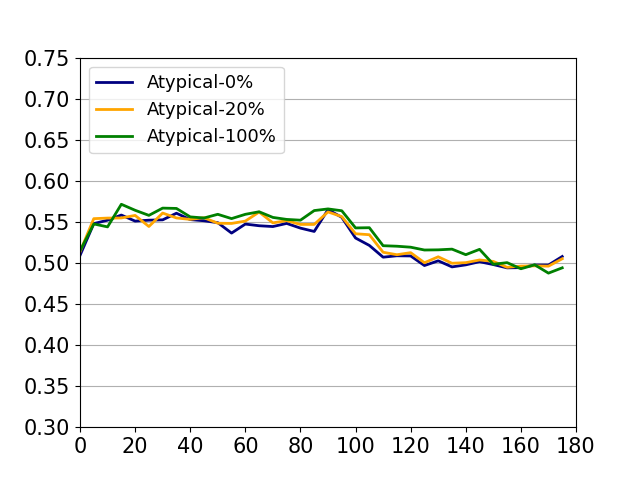
\includegraphics[width = 0.5\textwidth]{figures/dist_adv_cifar10_ResNet18.png}%
\hfill
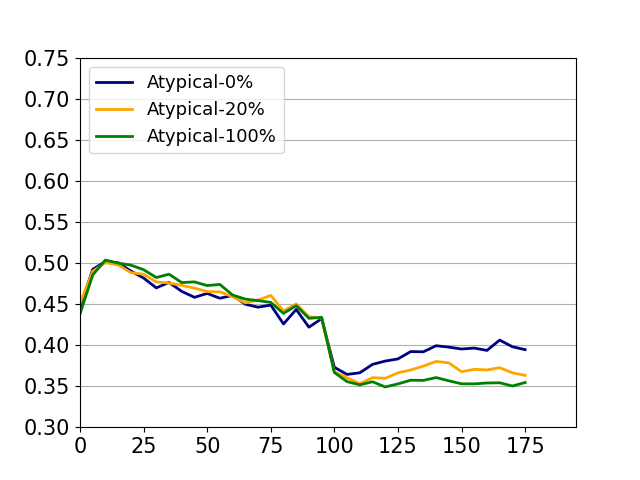
\includegraphics[width = 0.5\textwidth]{figures/dist_adv_cifar10_WRN28.png}
\end{minipage}
}
\caption{Classwise Cosine Distance of Output Representation of \textbf{Typical} Set of CIFAR10}
\label{fig:dist2}
\end{figure}


%%%%%%%%%%%%%%%%%%%%%%%%%%%%
\begin{figure}[h!]
\centering
\hspace*{-1cm}
\subfloat[Traditional ERM under ResNet32 (left), WRN28 (right).]{
\begin{minipage}[h]{0.55\textwidth}
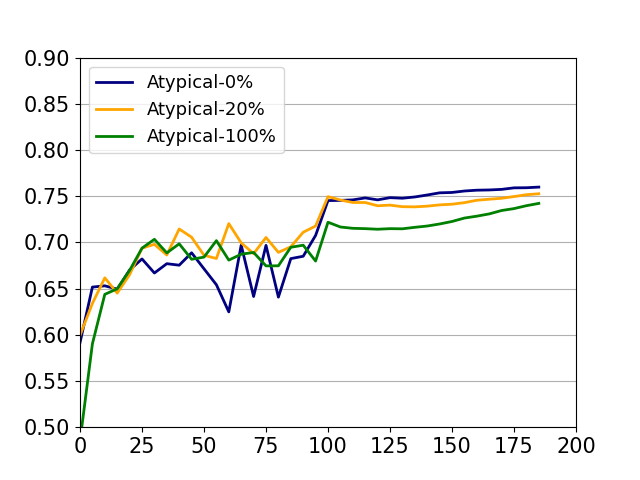
\includegraphics[width = 0.5\textwidth]{figures/dist_imagenet_ResNet18.png}%
\hfill
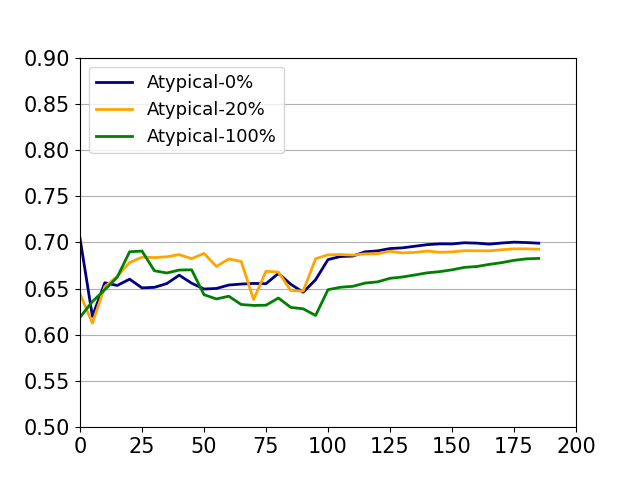
\includegraphics[width = 0.5\textwidth]{figures/dist_imagenet_WRN28.png}
\end{minipage}
}
\hspace*{-0.4cm}
\subfloat[Adv. Training under ResNet32 (left), WRN28 (right).]{
\begin{minipage}[c]{0.55\textwidth}
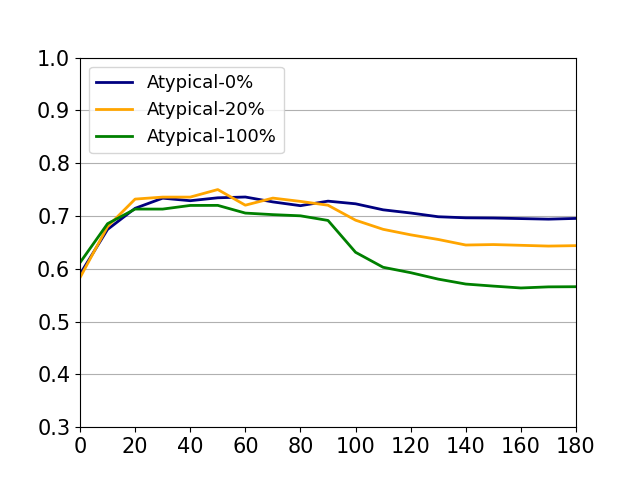
\includegraphics[width = 0.5\textwidth]{figures/dist_adv_imagenet_ResNet18.png}%
\hfill
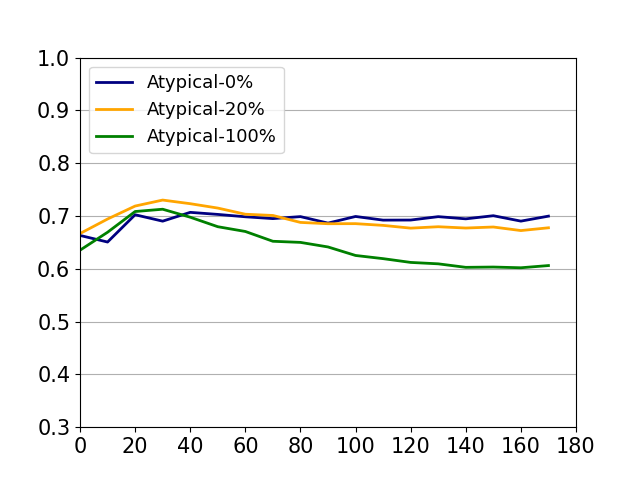
\includegraphics[width = 0.5\textwidth]{figures/dist_adv_imagenet_WRN28.png}
\end{minipage}
}
\caption{Classwise Cosine Distance of Output Representation of \textbf{Typical} Set of Tiny~ImageNet}
\label{fig:dist3}
\end{figure}


